\documentclass[12pt,a4paper]{article}
\usepackage[margin=2.5cm]{geometry}
\usepackage[utf8]{inputenc}
\usepackage[
    backend=biber,
    style=apa,
    citestyle=authoryear,
    sortcites=true
]{biblatex}
\setlength{\bibitemsep}{0.5em}
\addbibresource{references.bib}
\usepackage{parskip}
\usepackage{xcolor}
\usepackage{graphicx} % Add this package for including images
\usepackage{hyperref} % Add this package for hyperlinks
\usepackage{caption} % Add this package for caption customization
\usepackage{float}
\usepackage{titling} % For customizing the title page

\title{Asynchronous Synergy: A Study of Performance in Multi-Core Threading Across Programming Languages}
\author{Jonas Wolffrom}
\date{\today}

% Redefine the \maketitle command to include the logo
\renewcommand{\maketitle}{
  \begin{titlepage}
    \centering
    \vspace*{1cm}
    
    
\includegraphics[width=0.4\textwidth]{ruc_logo.png}\\[2cm]
    
    {\LARGE\bfseries\thetitle\par}
    \vspace{1.5cm}
    
    {\Large\theauthor\par}
    \vspace{1cm}
    {\large Supervisor: \par}
    {\large\textit{Henning Christensen}\par}   
    \vspace{1cm}
    
    {\large\thedate\par}
    \vfill
    
    {\large Roskilde University\par}
    {\large Department of Humanities and Technology\par}
    \vspace{0.5cm}
  \end{titlepage}
}

\begin{document}

\maketitle
\newpage

\begin{abstract}
This study investigates the performance characteristics of multi-core threading across four widely used programming languages: C, C\#, Java, and Python. As processor manufacturers shift from increasing clock speeds to adding more cores, the ability to effectively utilize these cores through software becomes increasingly important. We benchmark a simple counting algorithm on a quad-core system using language-specific threading implementations and measure the resulting performance improvements. Our findings reveal significant variations in threading efficiency, with Java achieving near-optimal utilization (382\% improvement), followed by C\# (304\%) and Python (204\%), while C with POSIX threads surprisingly demonstrated a performance decrease (76\% of single-thread speed). These results challenge conventional wisdom about low-level languages offering superior performance for parallel tasks and suggest that the quality of threading implementation is more critical than language abstraction level. The study concludes that while multi-core threading can approach theoretical scaling limits with proper implementation, achieving this potential depends heavily on sophisticated thread management systems that effectively bridge user-level and kernel-level scheduling. These insights help explain the diminishing returns experienced by consumers with high core-count processors and offer guidance for both developers seeking to better leverage parallel computing resources.
\end{abstract}
\newpage

\tableofcontents
\newpage

\section{Disclosure}

Any and all resources related to- and used in this study can be found here:

\begin{center}
    \href{https://github.com/X1las/AsSynergy}{https://github.com/X1las/AsSynergy}
\end{center}

Due to the amount of variables that can affect the performance of a CPU, the results of this study should be taken in comparison to each other, and not as a definitive measure of performance. It is encouraged to run the code snippets on your own machine to get a better understanding of the performance improvements that can be achieved with multi-core threading. Graphs in this paper were made using 'matplotlib' in a Jupyter notebook environment, the code for which can be found in the repository linked above.

Everything in this paper has been written by human hands, however some code snippets have been partially generated by AI, specifically Claude 3.7 Sonnet. Additionally, AI has been used for spell checking, sentence structure corrections, as well as text reductions, however everything has been checked by a human to make sure edits do not conflict with the cited theory, in addition to ensuring code snippets provided are correct and functional.

Lastly, this paper falls within the scope of the Humanities and Technology department at the University of Roskilde, as it aims to understand how multi-core threading is being used in society today, and how it can be improved. More specifically, it falls within the dimension of Technological Systems and Artifacts (TSA) as we take a look at computer systems at large, and how people are using them- as well as how concepts within them are understood.

\section{Introduction}

Quoted by \cite{Rauber2023}, "Moore’s law is an empirical
observation which states that the number of transistors of a typical processor chip
doubles every 18 to 24 months. This observation has first been made by Gordon
Moore in 1965 and has been valid for more than 40 years. However, the transistor
increase due to Moore’s law has slowed down during the last years" 

\citeauthor{Rauber2023} posits that the number of transistors on a microchip used to double rougly every two years, leading to an exponential increase in computing power. However they, in accordance with \cite{Mattson2014}, agree that this trend has been dwindling since some time around 2005, as a limit was reached on how many transistors could be placed on a single computer chip without overheating and damaging the circuitry. Even by utilizing the most advanced tricks and optimizations available, the performance improvements we are seeing annually as of 2023 are somewhere around 3.5\% faster CPU clock speeds \parencite[p. 11]{Rauber2023} which is a far cry from the 50\% annual increases we were seeing in the early 2000's \parencite[p. 11]{Rauber2023}. 

As a result of the processing speed ceiling, the focus has shifted from increasing the clock speeds of CPUs to adding more computational units to them. This has led to a rise in multi-core processors, which contain multiple processing units on a single CPU chipset, often referred to as "cores". These cores can execute multiple orders simultaneiously, which can lead to significant performance improvements in software applications. However, a discrepancy can be found in the communities that rely on these improvements. An article from IGN \parencite{Thomas2025} on picking optimal hardware for computer games describes it best:

\begin{quote}
    \textit{\textcolor{darkgray}{"While there are some PC games that love CPUs with a dozen or more cores, they’re few and far between. 
    Instead, finding an 8-core, 16-thread processor with a high clock speed and a lot of L3 Cache is going to get you further than just adding more CPU cores to the equation". }}
\end{quote}

A trend of diminishing returns can be seen, or rather felt on a consumer basis. Even people who purchase CPUs know to steer away from something that advertises a high amount of cores, as it's simply not worth it. Whereas the relationship between core-count and performance we should be seeing, in theory, should be an equivalence. It is evident that traditional single-core processors are opting out of the market in place of processors with more and more cores \parencite{Smith2023}, but the performance improvements are not being felt by the end-user.

\subsection{The Problem Area}

If multi-core threading is the future, then it is essential to understand why it is not delivering the expected performance improvements it has the potential to deliver. \cite[p. 12]{Rauber2023} mentions that simulations have shown that superscalar processors with up to four functional units yield substantial benefits over the use of a single functional unit. So in theory, it would seem there is great potential to gain from utilizing multiple cores. Some of it has been utilized according to \textcite{Thomas2025}, as we are talking about 8-cores as opposed to one, but it has taken us 20 years to get to this point.

As such, this study aims to address this question of why multi-core optimization is so difficult to accomplish, if and/or how it can be improved, and what the potential benefits of doing so are. 

\subsubsection{Research Question}

With the problem in mind however, there are limits to what can be achieved in such a short study, therefore we will be focusing mainly on threads and schedulers. The way to implement them, as well as how different programming languages handle them. This will be done by looking at the different threading libraries available in C, C\#, Java and Python, as well as the different ways in which they are scheduled.

The research question that we will be addressing is then as follows:

\begin{quote}
    \textit{What does multi-core threading offer in terms of performance improvements to different programming languages, and what stops us from utilizing its full potential?}
\end{quote}

This is the most pressing question we will try to answer, and to do so, we will have to answer these following sub-questions:

\begin{itemize}
    \item What is a parallel system, and how do threads help make them?
    \item How does one create threads in practice and what similarities are there between programming languages?
    \item What performance increases and deficits does multi-core threading incur?
    \item What are the challenges of multi-core threading, and how can they be overcome?
\end{itemize}

These questions should serve to answer the most pressing matters related to this study, namely what threads are, where they are used, how to make them and what it shows us in terms of performance. To these, we have composed two hypotheses on what we expect to find in this study:

\begin{itemize}
    \item[H1:] Threading is simple in theory, but difficult to apply in practice.
    \item[H2:] The performance improvements of multi-core threading do not exceed a doubling in performance.
    \item[H3:] Not all cores are fully utilized in multi-core threading.
\end{itemize}

The challenges of multi-core threading will be addressed in the discussion section, where we will look at the results of the benchmarks and how they relate to the research question, as well as affirm/debunk the hypotheses, but before that we will need to adress the limitations of this study, as well as the theoretical background that is necessary to understand the subject matter.

\subsubsection{Limitations}

This study is limited in its research and data-collection to only a handful of programming languages: C, C\#, Java and Python. This is due to limitations in time and resources, as well as the fact that these languages are some of the most commonly known programming languages in the field, hopefully leaving the readers with at least one language they are familiar with. This sample size should be sufficient to provide a good overview of how threading is implemented in general, as well as how it is used in practice. 

This being said, we will not linger on the specifics of each language, but rather focus on how the different threading libraries relate to each other, as well as highlight some key differences important to the overall topic of threads. This is to ensure that we can provide a comprehensive overview of the subject matter without getting bogged down in the details of each language.

Additionally, this study limits its scope to just Linux systems, more specifically Ubuntu, as this was the easiest method of collecting data. This is due to linux having a lot of built-in tools and easy-to-install features that allowed for easy programming in all 4 different languages. This is not to say that the theory is not applicable in other operating systems, in fact we encourage the reader to run and the code snippets on other environment to see if the results are similar- However, we will not be able to provide any data on this, as it was not part of the study.

\section{Asynchronous Systems}

To understand multi-core systems, we must differentiate between synchronous and asynchronous execution paradigms, which form the foundation for task distribution across processing units.

In single-core processing, operations follow a synchronous model where instructions execute sequentially \parencite[p. 118]{Johnson2015}. While straightforward, this approach leads to processor "idling" when waiting for I/O operations, creating a significant performance bottleneck, especially in I/O-bound applications.

\begin{quote}
    \textit{\textcolor{darkgray}{"It is much easier to reason sequentially, doing only one thing at a time, than to understand situations where many things occur simultaneously." ... "Thus, while we are "parallel processors", and we live in a world where multiple things happen at the same time, we usually reason by reduction to a sequential world."}} - \cite{Rajsbaum2020}
\end{quote}

This necessitates "context switching"\parencite[p. 4]{Rauber2023} between tasks, allowing the processor to alternate between different operations, creating the illusion of concurrency. Operating systems manage this through time-slicing, where each process receives a brief execution window.

\subsection{Subroutines and Coroutines}

Programmers typically interact with concurrency through subroutines (functions) \parencite{Pyeatt2020}, which encapsulate functionality for reuse across programs. Coroutines extend this concept by allowing suspension and resumption at specific points \parencite{DeMouna2009}, enabling a routine to "yield" control before completing execution. Unlike traditional subroutines, coroutines establish a collaborative relationship where control passes between routines that maintain their state between invocations.

Coroutines can be synchronous (waiting for completion before continuing) or asynchronous (returning immediately, allowing the calling code to continue). This suspension capability is expressed through 'yield' and 'resume' operations, enabling cooperative multitasking without requiring task completion.

Python demonstrates this with its async/await syntax:
\begin{verbatim}
import asyncio

async def main():
    print('Hello ...')
    await asyncio.sleep(1)
    print('... World!')

asyncio.run(main())
\end{verbatim}

The 'await' keyword marks where execution can be temporarily halted while waiting for an operation to complete, allowing other tasks to execute during this suspension.

When expanding to multiple processing units on the same chipset (a multi-core processor), we can maintain this synchronous approach for consistency or adopt an asynchronous model that allows processing units to operate with greater independence. The choice between these approaches often depends on the nature of the problem being solved, with data-intensive parallel applications favoring synchronous models that emphasize predictable behavior, while I/O-bound or service-oriented applications typically benefit from asynchronous models that maximize throughput by avoiding unnecessary blocking.

\subsection{Parallelism}

In practice, synchronous and asynchronous models rarely exist in their purest forms. Even highly parallel systems require synchronization mechanisms to coordinate access to shared resources\parencite[p. 95]{Rauber2023}. When multiple cores access the same memory locations, these operations must be coordinated, and the underlying hardware and operating system often introduce asynchronous behavior through context switching.

Parallelism refers to the ability to execute multiple tasks simultaneously across multiple processors or cores\parencite[pp. 4-5]{Rauber2023}. While concurrency is about managing multiple tasks regardless of simultaneous execution, parallelism specifically focuses on the simultaneous execution of multiple computations. This distinction is critical when designing systems that must scale effectively across multiple processing units.

Within this realm of paralelism, a few important terms are especially valuable for this paper, namely: "Degree of Parallelism" (DOP)\parencite[pp. 11-13]{Rauber2023}, "Load Balancing"\parencite[p. 5]{Rauber2023}, "Idle Time"\parencite[p. 5]{Rauber2023}, and "Parallel Execution Time" (PET)\parencite[p. 5]{Rauber2023}. These concepts are good to note, as they are often used to describe the performance improvements that can be achieved by using multiple cores in a program, or otherwise the reasons for why they are not being achieved.

\textbf{Degree of Parallelism} is a measure of how many tasks can be executed at the same time, and is often used to describe the performance improvements that a parallel system provides. This, in turn, coincides with the concept of "Potential Parallelism", which is the theoretical maximum degree of parallelism that a system can achieve. These two are often used to describe the performance improvements that a parallel system can provide, as well as what it is providing, making them useful means of benchmarking a parallel system's performance.

\textbf{Parallel Execution Time} quantitatively describe the time it takes for a parallel system to execute a given task. This execution time is measured across all functional units, or cores of a system, and can be used to give a tangible measure of the running time of a parallel program. This means that waiting times for memory fetching, writing and plain idle times are included in the measure. In terms of coding with multi-core threading, this means that "scheduling" time is included in the measure as well, as this is the time it takes for the operating system to assign tasks to different cores. This is important to note, as it means that the performance improvements of a parallel system are not just determined by the number of cores, but also by the efficiency of the scheduling algorithm used by the operating system.

Parallelism comes in four "Granularities"\parencite[p. 4, 114]{Rauber2023} which are often referred to as "Levels of Parallelism". These levels are: Instruction Level Parallelism (ILP), Statement Level Parallelism (SLP), Loop Level Parallelism (LLP), and Function Level Parallelism (FLP).

\textbf{Instruction Level Parallelism} refers to the ability of a system to execute multiple processor instructions simultaneously\parencite[pp. 115-116]{Rauber2023}. 'Instructions' refer to the simplest logic or arithmetics that can be executed at the transistor level of the processor. ILP is often used in modern processors to improve performance by allowing multiple instructions to be executed at the same time, breaking down complex operations into small and simple instructions that can be executed in parallel. 

\textbf{Statemwnt Level Parallelism} refers to the ability of a system to execute multiple statements simultaneously\parencite[pp. 114]{Rauber2023}. This granularity is just a bit coarser than ILP, and refers to executing multiple groups of instructions in parallel.

\textbf{Loop Level Parallelism} refers to the ability of a system to execute multiple iterations of a loop simultaneously\parencite[pp. 118-121]{Rauber2023}. This is achieved by looking at sequential loops, and identifying independent iterations that subsequentially can be executed in parallel. This relates to Data Parallelism\parencite[pp. 116-118]{Rauber2023} as well, as it relies on the ability to execute the same operation on multiple data elements in the same dataset, often as an array. 

\textbf{Function Level Parallelism} refers to the ability of a system to execute multiple tasks simultaneously\parencite[pp. 114, 121-122]{Rauber2023}. This is achieved by identifying subsequent parts of a program that can be executed independently of each other and can be anythin from single statements to functions. This is synonymous with the term "Thread Level Parallelism" (TLP)\parencite[pp. 27-36]{Rauber2023}, which is often used to describe the performance improvements that can be achieved by using multiple threads in a program. However, to achieve TLP, it is necessary to utilize an abstraction of Threads, which vary in shape and size depending on a lot of factors, such as programming language and operating system, which we will look at in the following section.

\section{Threading}

Threads have been addressed varyingly in the literature throughout this paper and the documentation about to be presented especially, but generally speaking, and according to \cite[4, 27]{Rauber2023}, threads can be understood as a sequence of instructions that can be executed independently of other threads. These threads share the same memory space within a process' dedicated memory space, allowing them to communicate and share data with each other without the need for inter-process communication. This shared memory model is what identifies threads from processes, but as we will see later, the definition can be more nuanced.

The reason why subroutines and coroutines relate to this topic, is because a thread is, in practice, a coroutine, and as will be demonstrated later, are usually created by passing a subroutine as a thread within different languages. Threads can be suspended mid-execution as well as yield to other processes akin to coroutines, such that the processor it runs on always has something to do. Multi-threading is an achievment that can be achieved in single-core systems as well, by continuous context switching between different threads\parencite{Rauber2023} we achieve Concurrency. This concurrency does not negate Parallelism, as both can be achieved by context switching between different threads on multiple cores, allowing for a high degree of TLP.

\subsection{Kernel- and User Threads}

Threads are divided into two main categories: "User-threads" and "Kernel-threads" \parencite[p. 27]{Rauber2023}. User-level threads being the threads closest to the user/programmer, and kernel threads being the threads that are created and managed by the operating system itself.

\begin{quote}
    \textit{\textcolor{darkgray}{"The kernel threads are mapped by the operating system to processors or cores for execution. User threads are managed by the specific programming environment used and are mapped to kernel threads for execution. The mapping algorithms as well as the exact number of processors or cores can be hidden from the user by the operating system."}} - \parencite[p. 27]{Rauber2023}
\end{quote}

These user-threads are managed by the afforementioned programming languages used, and are mapped to kernel threads for execution. This means that the operating system is responsible for managing the execution of kernel threads, while user threads are managed by the particular programming environment used. This allows for a high degree of flexibility and control over the execution of threads, but it also means that the performance of user threads can be affected by the performance of the kernel threads they are mapped to, as well as the mapping algorithms used by their own programming environment. This is important to note, as it adds additional layers of complexity to measuring the performance of threads, as the affected performance of user threads can vary depending on the operating system and programming environment used.

\subsection{Scheduling}

Schedulers are usually thought of as the operating system's way of managing the execution of threads, and are responsible for determining which threads should be executed at any given time. However, this can further be broken down to user-level schedulers and kernel-level schedulers\parencite[pp. 154-155]{Rauber2023}.

User-level schedulers are implemented in the programming language itself, and are responsible for mapping their own threads to kernel threads for execution. This means that the user-level scheduler is responsible for which of its' threads should be executed at any given time, and what kernel thread they should be mapped to. Kernel-level schedulers, on the other hand, are OS Schedulers that are responsible for managing the execution of kernel threads\parencite[pp. 155-156]{Rauber2023}. They don't have any knowledge of user-level threads, and are only responsible for managing the execution of kernel threads. This means that the kernel-level scheduler is responsible for which kernel threads should be executed at any given time, and more importantly what Processor they should be executed on, dividing up the workload across the available cores in the system. 

The way that these schedulers map can be divided into several categories as defined by \citeauthor[pp. 155-156]{Rauber2023}:

\textbf{N:1 Mapping} or 'Many to One' mapping is the simplest form of mapping, where multiple user threads are mapped to a single kernel thread. This means that the programming environment's thread user-level scheduler is responisble of managing the execution of multiple user threads, and that the kernel-level scheduler is responsible for managing the execution of a single kernel thread.

\textbf{1:1 Mapping} or 'One to One' mapping is the more complex form of mapping, where each user thread is mapped to a single kernel thread. This means that the programming environment's thread scheduler is not responsible for managing the execution of multiple user threads, leaving that to the kernel-level scheduler.

\textbf{N:M Mapping} or 'Many to Many' mapping is a hybrid approach that combines the two previous approaches, wherein multiple user-level threads can be mapped to a selection of kernel-level threads. This means that both the programming environment's thread scheduler and the kernel-level scheduler are responsible for the managing and execution of multiple user threads, allowing for a high degree of flexibility and control over the whole process at user-level. This is often used in systems that require a high degree of parallelism, as it allows for multiple user threads to be executed simultaneously on different kernel threads.

\section{Threading in different languages}

In order to create threads in a program, we often use a threading library that is provided by the programming language. Usually, this is done by creating a function or subroutine that pertains the code to be run independently, using the threading library to pass the function to its own thread. This will become clearer in the following sections, where we will be looking language specific methods of threading in the afforementioned programming languages, starting with the POSIX library, as it relates to both C and Python.

\subsection{Posix}

POSIX, or "Portable Operating System Interface"\parencite{GNUPOSIX,POSIXDocs}, is a set of operating system standards that include features such as a shell, file system, and threading. It is a standard for multi-threading and comes pre-installed with the GCC compiler\parencite{GNUPOSIX} used for this study. POSIX carries a certain level of overhead, as it is not exclusively a threading library, nor is it a library made for C specifically. It is a standard that is implemented in C, but languages such as Python utilize it as well when using the 'multiprocessing' library. When used in this context of multi-threading, it is referred to as 'pthreads', and will be referred to as such in this paper.

Pthreads are essentially user-threads that are created and managed by the POSIX scheduler, this scheduler is responsible for mapping user-level threads to kernel-level threads for execution. In C, scheduling priority and policies can be changed to one of three as per \cite[pp. 359-360]{Rauber2023}:

\begin{itemize}
    \item \textbf{SCHED\_FIFO}: A first-in-first-out scheduling policy that allows threads to run in the order they were created, with no preemption.
    \item \textbf{SCHED\_RR}: A round-robin scheduling policy that allows threads to run in a cyclic order, with preemption after a certain time slice.
    \item \textbf{SCHED\_OTHER}: The default scheduling policy that is used by the operating system, which is usually a combination of FIFO and RR.
\end{itemize}

For further reading on the POSIX standard, for further reading see \fullcite{Stevens2005} on programming in UNIX environments, as well as \fullcite{Harbour2003} an older article on posix functionality that still holds relevance.

\subsection{Threading in C}

As previously mentioned, in order to accomplish multi-core threading in C we make use of the POSIX library, which comes pre-installed in the GCC compiler used to compile C-code on unix systems. This library provides access to pthreads, which we can easily invoke by including the header file 'pthread.h' in our code:

\begin{verbatim}
#include <pthread.h>
\end{verbatim}

After this, we can create a thread by first making a pthread variable to pass on to the pthread\_create function, which takes a function pointer as its first argument. This function pointer is the function that will be executed in the new thread, and it must have a specific signature in order to be used with pthreads. The signature is as follows:

\begin{verbatim}
void *function_name(void *arg) {
    // Code to be executed in the new thread
}

int main() {
    pthread_t thread;
    pthread_create(&thread, NULL, function_name, NULL);

    return 0;
}
\end{verbatim}

Posix provides the ability to work with multi-core systems by default, unless the used specifies something different by declaring "AFFINITY":

\begin{verbatim}
#include <pthread.h>
#include <sched.h>
#include <stdio.h>

void *function_name(void *arg) {
    // Code to be executed in the new thread
    return NULL;
}

int main() {
    pthread_t thread;
    cpu_set_t cpuset;

    // Set the CPU affinity for the thread
    CPU_ZERO(&cpuset);
    CPU_SET(0, &cpuset); // Set the thread to run on CPU 0

    pthread_create(&thread, NULL, function_name, NULL);
    pthread_setaffinity_np(thread, sizeof(cpu_set_t), &cpuset);

    pthread_join(thread, NULL); // Wait for the thread to finish

    return 0;
}
\end{verbatim}

What this code does is create a thread that will run on CPU 0, and then wait for the thread to finish before exiting the program. This is a simple example of how to use pthreads to create a thread in C, but it is important to note that this is not the only way to do it. There are many other functions and options available in the pthreads library that can be used to create and manage threads, such as pthread\_join, pthread\_detach, and pthread\_cancel. These functions allow for more advanced thread management, such as waiting for a thread to finish, detaching a thread from the main process, or canceling a thread that is no longer needed. For further reading on the pthreads library, see the official documentation: \fullcite{PthreadDocs}.

\subsection{Threading in C-Sharp}

C\# just like C, is a compiled language that comes from the C language family like Python \parencite{PythonFAQ}, however where it differs is its striking resemblance to Java and its use of object oriented programming. To get started with threading in C\#, the process might look somewhat different in other environment, as we will be using the .NET 8 framework for Unix, which comes pre-built with a thread class. This class is ready for use on install, and is easily utilized by instantiating a thread object\parencite{CSThreadClass} and passing it a function to run:

\begin{verbatim}
class thread_example {

    static void MyThreadFunction() {
        // Code to be executed in the new thread
    }

    static void Main(string[] args) {
        Thread thread = new Thread(new ThreadStart(MyThreadFunction));
        thread.Start();
    }
}
\end{verbatim}

Not too dissimilar from how it was carried out in C, we create a function wherein we write the code to be executed in the new thread, and then we create a thread object that takes a function pointer as its argument. If we look at how C\# threads are scheduled however, we see that it draws a clear distinction between threads and processes\parencite{White2020}. Processes are dedicated spaces of memory within a program, wherein threads are the sole executers of tasks. In regards to the afforementioned "affinity" of threads, C\# extends this by providing not just affinity for the threads themselves, but also an overall process affinity to induce priority of programs. This is done by invoking 'SetPriorityClass' within the code, as well as 'SetThreadPriority' for individual thread priority\parencite{CSThreadPriority}. This allows for a high degree of control over the execution of threads, and gives the programming environment the ability to schedule user-level threads.

This is a simple example of how to use threads in C\#, it includes further functionality that we won't get into depths about in this study, but further reading can be found in the official documentation: \fullcite{CSThreadClass} as well as this article on its implementation: \fullcite{Wagner2022}. In addition, it is possible to set the CPU affinity of a thread in C\# just like in C, but this is not as straightforward, see this documentation for more information: \parencite{CSProcessorAffinity}.

\subsection{Threading in Python}

Threading in python is carried out in a handful of ways, but the most common way is to use the 'threading' library\parencite{PythonThreading}, which comes pre-installed with Python:

\begin{verbatim}
import threading

def my_thread_function():
    # Code to be executed in the new thread
    pass

thread = threading.Thread(target=my_thread_function)
thread.start()
\end{verbatim}

This is again a simple example of how to use threads, but it is important to note that due to the Global Interpreter Lock (GIL) in Python, native threads can only run on a single core\parencite{PythonGIL}. This doesn't mean there are no ways of achieving multi-core threading in Python, as there are libraries such as 'multiprocessing' that allow for the creation of multiple processes that can run on different cores:

\begin{verbatim}
import multiprocessing

def my_process_function():
    # Code to be executed in the new process
    pass

thread = multiprocessing.Process(target=my_process_function)
thread.start()
\end{verbatim}

Despite being labelled as processes, these are still threads as they utilize run on POSIX under the hood\parencite{PythonMultiprocessing}, and are therefore still subject to the same limitations as pthreads. But even so, multi-core threading can be achieved in Python with relative ease, however it's difficult to notice the performance improvements as the GIL is still present\parencite{PythonGIL}. This means that even though we are creating multiple processes, they are still limited by the GIL, and therefore cannot take full advantage of multi-core systems. This is an important consideration when using Python for multi-core threading, as it can lead to performance issues if not handled correctly. For further reading on the threading library, see the official multiprocessing documentation: \fullcite{PythonMultiprocessing}

\subsection{Threading in Java}

Java Standard Edition (JSE) comes with a built-in threading library\parencite{JavaThreadClass}, usually this functionality is accomplished by inheritance, extending a class from 'Thread' and including a 'run' method that contains the code to be executed in the new thread:

\begin{verbatim}

class MyThread extends Thread {
    public void run() {
        // Code to be executed in the new thread
    }
}

public class Main {
    public static void main(String[] args) {
        MyThread thread = new MyThread();
        thread.start();
    }
}
\end{verbatim}

This is slightly different from other languages, as it uses inheritance to create a new thread class that extends the Thread class. This means that the thread objects created from this class will have all its methods and properties included, meaning we don't have to pass a function pointed to the thread object before running it, instead we just call the 'start' method on the thread object. In terms of multi-core threading, Java Virtual Machine (JVM) is able to utilize multiple cores in a program, as they are allotted a pool of Kernel Threads to operate with.

In addition to these, Java includes 'Virtual Threads' and 'Platform Threads'\parencite{JavaVirtualThreads} in their development kit. Virtual Threads are user threads that are managed by the JVM, and are mapped to platform threads for execution, foregoing being bound to a single kernel thread. Platform Threads are a little more complex, as they are essentially kernel threads but with a java wrapper around them, allowing the JVM to manage them more easily. This means that the JVM is responsible for managing the execution of platform threads, while virtual threads are managed by the JVM itself. This allows for a high degree of flexibility and control over the execution of threads, but it also means that the performance of virtual threads can be affected by the performance of the platform threads they are mapped to, as well as the mapping algorithms used by the JVM.

For more information on the Java threading library, see the official documentation: \fullcite{JavaThreadClass,JavaVirtualThreads}.

\section{Multi-Core Threading Benchmarks}

Before we get into the benchmarks of the different programming languages, it is important to disclose that the data was collected on a computer running Ubuntu 24.04.2 LTS with an intel Core i5-4460 CPU @ 3.2GHz, with 4 cores and 4 threads. The time measured was done so with various clocking methods depending on the programming language over the course of 5 runs, with the average time being taken as the final result. The code snippets used for the benchmarks can be found in the appendix.

For each experiment, we made sure to check that all four cores were being utilized by the program using the built in System Monitor in Ubuntu. This was of course done as a separate process, as the System Monitor itself is a program that runs on the same system, and therefore would interfere with the results of the benchmarks. All the numbers were manually recorded and then averaged out to get the final results. 

\subsection{Data Collection Process}

To begin with, we clocked the time it took to execute a simple count from 1 to 1 billion in the various languages to get a frame of references. This proved especially difficult for Java, as the JIL converts commonly used methods to bytecode to optimize the execution time. This meant that to get a proper benchmark we had to disable the JIT compiler by using the '-Xint' flag, which in turn made the execution time of Java significantly slower than the other languages, with the exception of Python.

This was done by simply looping from 1 to 1 billion using a for loop, recording the time before and after the loop, subtracting the two times to get the time for the execution to finish. This was repeated in each of the languages, proving no troubles until we got to the asynchronous benchmarks.

When it came to the asynchronous benchmark, a lot of things had to be taken into account, as different languages use different methods of threading, as well as multi-core threading. Java was especially different, as common examples shows it instantiating an object of the class inside itself, which was not the case in other languages as seen in the appendix. 

Every threading program followed the same trend/structure, where we first created a function which was subsequentially sent to a user-thread, then the programming environment and the OS handled the rest "under the hood". This meant that we didn't have to worry about the specifics of how to map the threads ourselves, but it also meant we had no idea how the threads were being scheduled. Neither did we know what cores they were being assigned to, along with how often context switching was happening both between the kernel threads as well as between the user threads. 

\subsection{Performance Results}

As expected, most of the time the results of running the code snippets on multiple cores were significant performance increases when compared to the single core. This makes sense, as evidently four cores are faster than one, however some of these results were quite surprising:

\begin{figure}[H]
    \centering
    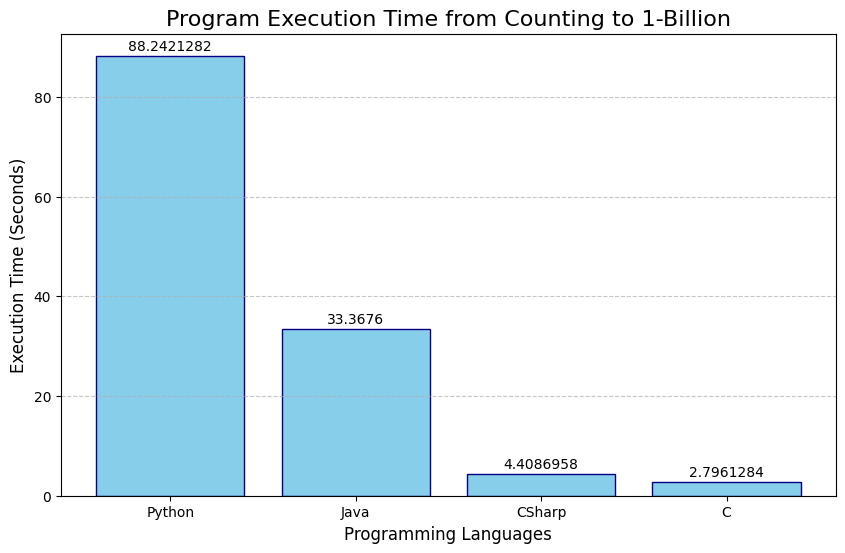
\includegraphics[width=0.8\textwidth]{../sync_records/sync_exec_times.png}
    \captionsetup{font=small, justification=centering}
    \caption{Execution time comparison of different programming languages running synchronously when counting from 1 to 1-billion.}
    \label{fig:sync-exec-times}
\end{figure}

The synchronous execution results above benchmark the time it took to compute the same task in each of the language. We saw expected results within most of the languages, with python having an average run time of 88 seconds, Java at 33, C\# 4 and C at just a little below 3 seconds. There was not much to note in these results, other than Java operating surprisingly slow when not using the JIT compiler.

\begin{figure}[H]
    \centering
    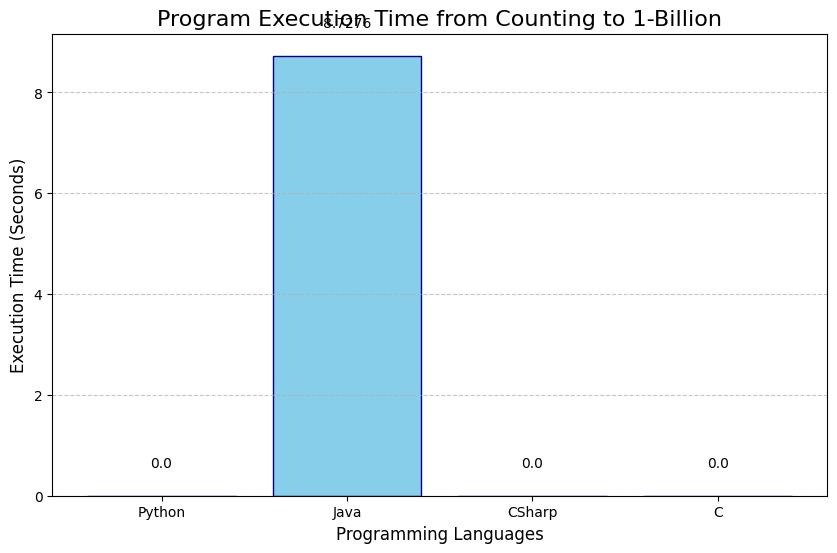
\includegraphics[width=0.8\textwidth]{../async_records/async_exec_times.png}
    \captionsetup{font=small, justification=centering}
    \caption{Execution time comparison of different programming languages running asynchronously with multi-threading when counting from 1 to 1-billion.}
    \label{fig:async-exec-times}
\end{figure}

The multi-core execution results reveal a greater deal about the efficiency of the different programming languages however, as there was a big shift. Python was able to achieve a time of 43 seconds on average which amounts to a little more than twice the performance increase. Java was able to achieve an astounding 8.7 seconds, a little less than 4 times the performance increase. C\# was able to achieve an average time of 1.44 seconds, surprassing the performance of C, which was able to achieve an average time of 3.66 seconds, a significant reduction in performance.

\begin{table}[H]
    \centering
    \begin{tabular}{|l|c|c|c|}
        \hline
        Language & Single Core (s) & Multi-Core (s) & Performance Increase (\%) \\
        \hline
        Python & 88.242 & 43.176 & 204.377\% \\
        Java & 33.368 & 8.728 & 382.310\% \\
        C\# & 4.407 & 1.449 & + 304.141\% \\
        C & 2.796 & 3.666 & 76.268\% \\
        \hline
    \end{tabular}
    \captionsetup{font=small, justification=centering}
    \caption{Execution times of different programming languages when counting from 1 to 1-billion, both single-core, multi-core and performance increases.}
    \label{tab:exec-times}
\end{table}

When looking at these numbers for C, the first thought is that something must have gone wrong with the multi-core scheduling, as it got slower when attempting to run on multiple threads, but the System Monitor confirms that all four cores were being fully utilized, so then what could the reason be for this?

\section{Analysis}

Looking at the benchmark results, several patterns emerge in how different programming languages utilize multi-core threading. The performance metrics reveal significant variations that can be attributed to each language's threading implementation and runtime environment characteristics.

\subsection{Threading Implementation Efficiency}

Java and C\# demonstrate comparable performance improvement patterns, with both languages achieving substantial speedups when executing on multiple cores. Java achieved an impressive 382\% performance increase, while C\# reached a 304\% improvement. These gains can be traced to their similar threading architectures, as both languages employ a sophisticated runtime environments (JVM and .NET respectively) that include built-in thread management systems at user-level.

Python's performance increase of 204\% is notable but more modest, likely reflecting the limitations imposed by the Global Interpreter Lock (GIL). Despite using the multiprocessing library to bypass the GIL, Python still shows performance constraints compared to Java and C\#. This aligns with expectations given Python's higher-level abstraction and interpreter-based execution model.

The surprising finding is C's performance decrease at 76\% of the single core execution when using multiple threads. This counter-intuitive result requires further examination, especially considering that the system monitor confirmed all four cores were being utilized. The POSIX threading implementation in C appears to introduce overhead that outweighs the potential benefits of parallel execution for this specific benchmark task.

\subsection{Thread-to-Core Mapping}

In all these test cases, we maintained a consistent approach of creating exactly four threads to match the four available CPU cores. The system monitor consistently showed full CPU utilization across all cores, indicating successful user-thread-to-kernel-thread mapping. This could suggests a 1:1 scheduling model for these small-scale test cases, where each user thread is mapped to a kernel thread, which in turn is allocated to a physical core. But seeing as the performance of C was remarkably worse than expected, it might be that the POSIX scheduler is the only one to utilize 1:1 mapping, whereas Java and C\# use an N:M mapping, potentially allowing for more performance by having a larger pool of kernel threads to draw from by clever user-thread scheduling.

\subsection{Performance Scaling Analysis}

Most notably, Java achieved an impressive 382\% performance improvement, coming remarkably close to the theoretical maximum of 400\% (representing perfect utilization of all four cores). This suggests that Java's thread management system is exceptionally efficient at utilizing multiple cores for this particular benchmark task. C\# also performed admirably with a 304\% improvement, while Python achieved a full doubling with 204\%.

The near-linear scaling observed in Java indicates that its threading implementation has minimal overhead, allowing it to achieve close to perfect parallelism. This is particularly impressive considering the complexity involved in coordinating multiple threads across cores. The fact that Java can reach 95.5\% of the theoretical maximum efficiency suggests that well-designed thread management systems can effectively overcome many of the traditional barriers to parallel performance.

For the simple task of counting numbers used in our benchmark, the degree of parallelism is naturally high since the work can be easily divided among threads with minimal interdependence. This scenario is ideal for testing the raw capability of threading implementations without the complications of shared memory access or synchronization issues. The near-optimal performance of Java demonstrates that under ideal conditions, modern threading implementations can approach theoretical maximum efficiency.

The stark contrast between Java's near-perfect scaling and C's disappointing 76\% relative performance (a 24\% slowdown) highlights how critical the implementation details are to threading performance. Despite all languages utilizing all four cores according to system monitoring, their efficiency in doing so varies dramatically.

\subsection{Overhead Factors}

Based on the theory and our results, we can say for certain that these factors are generally responsible for the overhead in multi-threading performance:
\begin{itemize}
    \item Thread creation and initialization costs
    \item Context switching between threads
    \item Scheduling decisions at both user and kernel levels
    \item Memory access patterns and cache coherence
    \item Thread synchronization mechanisms
\end{itemize}

For our test execution specifically, the overhead for shared memory as well as synchronization is minimal, as the counting task is inherently isolated. However there are uncertainties whether libraries introduce additional synchronization or locking mechanisms that could impact performance.

In C specifically, the POSIX threading library appears to introduce disproportionate overhead, judging solely by the performance outlier of Python and C, as they both rely on POSIX to schedule threads on Unix systems. As a general-purpose system interface rather than a C-specific library, POSIX may not be optimized for the particular scheduling needs at user-level that C\# and Java exhibit.

This could of course also be due to the fact that C is a lower-level language, and therefore has less abstraction to work with when it comes to threading, and that the fault lies with us as the programmers, as we did not implement them in the correct way for this specific case. 

\section{Discussion}

The significant variations in multi-threading performance between languages raise important considerations for software development. Java and C\# demonstrate the advantages of purpose-built threading systems integrated with their respective runtime environments. These languages have clearly benefited from decades of optimization for concurrent execution models.

This stands opposed to the poor performance of C with POSIX threads, challenging the conventional wisdom about lower-level languages always providing better performance. This finding suggests that the abstraction level of a language may be less important for multi-threading performance than the design and optimization of its threading library and runtime environment. Java, despite its reputation for overhead due to the JVM, demonstrates excellent thread scaling, likely due to its extensive optimization for enterprise multi-threaded applications.

\subsection{User-Level vs. Kernel-Level Thread Management}

Our findings highlight the complex relationship between user-level and kernel-level thread management. The near-perfect scaling of Java (382\% improvement on a quad-core system) suggests that its thread management system has solved many of the traditional challenges in bridging application-level threading needs with kernel-level scheduling. This remarkable efficiency indicates that Java's sophisticated user-level scheduling works almost seamlessly with the underlying OS scheduler.

The substantial gap between Java's 382\% and C's 76\% performance with the same number of cores and threads strongly suggests that the mapping strategy between user and kernel threads is critical. Java's virtual threads, which intentionally decouple application threading from kernel threading, appear to offer a superior approach. By allowing many lightweight user threads to be divided amongst a smaller pool of kernel threads, this model delivers nearly optimal resource utilization while maintaining programming simplicity.

This raises a fundamental question about the design of threading systems: is the two-level approach (user and kernel) optimal, or does it introduce unnecessary complexity and overhead? Java's virtual threads, which intentionally decouple application threading from kernel threading, represent one approach to addressing this issue. By allowing many lightweight user threads to be divided amongst a smaller pool of kernel threads, this model potentially offers better resource utilization while maintaining programming simplicity.

\subsection{Benchmark Limitations and Ecological Validity}

The simple counting task used in our benchmarks represents a near-ideal case for parallelization—it requires minimal shared memory access and has perfect divisibility. In real-world applications, workloads typically involve more complex dependencies, shared resource access, and varying computational intensities. Nevertheless, our benchmark provides valuable insight into the theoretical upper bounds of performance improvements through multi-threading.

If even this highly parallelizable task cannot achieve linear scaling with the number of cores, more complex real-world applications will likely face even greater challenges in effectively utilizing multiple cores. This suggests that the "free lunch" of performance improvement through increasing core count has definite limitations, supporting the observations from consumer experience noted in our introduction.

\subsection{Revisiting Our Hypotheses}

Returning to our initial hypotheses:

\textbf{H1: Threading is simple in theory, but difficult to apply in practice.}
Our theory and analysis somewhat disagrees with this notion. It was surprisingly easy to apply in practice, as all languages provided a simple way to create threads and run them concurrently across multiple cores right out of the box. In addition to this, the principles of threading were rather straight forward in essence, but it seems quite difficult to figure out how scheduling is carried out, as it varies so much between languages and operating systems. 

\textbf{H2: The performance improvements of multi-core threading do not exceed a doubling in performance.}
This hypothesis is firmly debunked by our results. Java achieved a 382\% improvement and C\# reached 304\%, both far exceeding a mere doubling of performance. Even Python, with its GIL limitations, managed a 204\% improvement. Only C failed to show positive scaling. These results demonstrate that with proper implementation, multi-threading can approach the theoretical maximum improvement equal to the number of cores.

\textbf{H3: Not all cores are fully utilized in multi-core threading.}
Our findings debunk this hypothesis entirely, as we saw both significant performance improvements and full utilization of all cores through the system monitor. Despite our initial concerns about not actually seeing any use of more cores than one, we were able to confirm they all were being utilized to their fullest.

\subsection{Implications for Software Development}

For developers, these findings suggest several practical considerations:

\begin{enumerate}
    \item \textbf{Language selection matters for parallel performance}: The significant variations between languages indicate that the choice of programming language and its threading implementation can substantially impact the ability to leverage multi-core architectures.
    
    \item \textbf{Thread count should match workload characteristics}: Simply creating threads equal to the number of available cores may not yield optimal performance, particularly for workloads that differ from our compute-bound benchmark.
    
    \item \textbf{Threading overhead must be considered}: The performance decrease in C demonstrates that threading introduces overhead that can outweigh benefits for certain applications or implementations.
    
    \item \textbf{Threading abstractions provide value}: The superior performance of Java and C\# suggests that higher-level threading abstractions, despite adding a layer between the programmer and the hardware, can result in better utilization of multi-core systems through optimized scheduling and resource management.
\end{enumerate}

These implications challenge the notion that increasing parallelism through more cores automatically translates to proportional performance improvements. The relationship between core count and performance is mediated by numerous factors, including language design, threading implementation, workload characteristics, and operating system scheduling policies.

\section{Conclusion}

Our investigation into multi-core threading across different programming languages reveals several key insights that directly address our research question: "What does multi-core threading offer in terms of performance improvements to different programming languages, and what stops us from utilizing its full potential?"

In terms of performance improvements, our benchmarks demonstrate that multi-core threading can offer substantial gains, with Java achieving a remarkable 382\% improvement—nearly reaching the theoretical maximum of 400\% on our quad-core system. C\# followed with 304\%, and even Python managed 204\% despite its GIL limitations. These results convincingly demonstrate that well-implemented threading can approach almost linear scaling with the number of cores. This directly answers our third sub-question regarding performance increases and deficits across languages.

Addressing our first sub-question about parallel systems, we've shown that a parallel system is one that can execute multiple instructions simultaneously across processing units. Threads serve as the fundamental building blocks of such systems by providing independent execution contexts that share memory space. Our benchmarks confirm that threads effectively enable parallelism, though their implementation efficiency varies significantly by language.

For our second sub-question about thread creation in practice, we've demonstrated that while the basic pattern of defining a function and passing it to a threading mechanism is common across languages, implementation details differ considerably. Java uses class inheritance, C\# and Python use function references, and C uses function pointers with specific signatures. Despite these syntactic differences, the underlying concept remains consistent, encapsulating executable code that can run independently. These similarities made our cross-language comparison possible, whilst the differences in implementation quality explained much of the performance variation.

What prevents full utilization—addressing our fourth sub-question about challenges appears primarily related to implementation quality rather than fundamental limitations. Java's near-perfect scaling suggests that the theoretical ceiling is attainable with proper design. The stark contrast with C's poor performance (76\% of single-threaded speed) highlights that threading implementation quality is the critical factor in achieving multi-core benefits. Challenges include overhead from thread creation and management, inefficient scheduling algorithms, and suboptimal mapping between user-level and kernel-level threads.

For the field to advance, we need better standardization of threading models across languages, improved debugging tools for thread visualization, and more transparent control over how threads are scheduled at both user and kernel levels. Without addressing these challenges, the full potential of multi-core architectures will remain partially untapped, continuing the trend of diminishing returns from increasing core counts in consumer hardware.

\section{Future Work}

Future research in this area could productively pursue several directions:

\textbf{Scalability at High Core Counts:} Investigating how traditional multi-core threading scales beyond the quad-core level and see how performance changes with commercially available CPUs that range all the way above 64 cores. This could help identify whether the performance ceiling observed in our benchmarks is a fundamental limitation of current threading models or if it can be overcome with more sophisticated scheduling techniques.

\textbf{Parallel Systems at Instruction Level:} Exploring how parallelism can be achieved at the instruction level, such as through vectorization or SIMD (Single Instruction, Multiple Data) techniques. This could help identify whether there are opportunities to improve performance by optimizing how individual instructions are executed in parallel, rather than relying solely on multi-threading.

\textbf{Identifying Bottlenecks in E-core and P-core Architectures:} Investigating how different core architectures, such as E-cores (Efficiency cores) and P-cores (Performance cores), impact multi-threading performance. This could help identify whether there are opportunities to optimize thread scheduling and resource allocation based on the specific characteristics of different core types, and whether schedulers already take these into consideration. 

\textbf{Power Efficiency and Thermal Management:} Examine how multi-threading at the higher core counts impacts power consumption and thermal management. As core counts increase, power efficiency might become a critical factor. If multi-threading fully utilizes all computing cores, what can be expected in terms of power consumption and heat generation? This could lead to insights on how the energy grid might be affected in the future, as well as see what can be done to mitigate these effects.

\textbf{GPU Core Parallelism:} Investigate how GPU's utilize their high core count to aid in large scale parallel computing tasks, and whether similar techniques can be applied to CPU multi-threading or vice-versa. In addition, looking at how CPUs and GPUs communicate with multiple cores on both ends working independently and whether blocking operations can be avoided or where they appear on both ends.

By addressing these areas, future work could help bridge the gap between theoretical parallel computing potential and practical performance improvements, ultimately enabling software to more effectively utilize the multi-core architectures that now dominate computing hardware.

\clearpage
\section{References}
\printbibliography
% Ensure Biber is run to resolve undefined references

\clearpage
\appendix
\section{Benchmark Execution Times}

\subsection{Synchronous Execution Times}

\begin{table}[H]
    \centering
    \begin{tabular}{|l|c|c|c|c|c|c|}
        \hline
        \textbf{Language} & \textbf{Run 1} & \textbf{Run 2} & \textbf{Run 3} & \textbf{Run 4} & \textbf{Run 5} & \textbf{Average} \\
        \hline
        C & 2.837 & 2.799 & 2.762 & 2.766 & 2.816 & 2.796 \\
        C\# & 4.410 & 4.418 & 4.390 & 4.382 & 4.443 & 4.409 \\
        Java & 30.3 & 30.448 & 30.346 & 30.178 & 30.566 & 30.368 \\
        Python & 86.742 & 86.754 & 92.835 & 86.853 & 88.027 & 88.242 \\
        \hline
    \end{tabular}
    \caption{Synchronous execution times (in seconds) for each language over 5 runs when counting from 1 to 1 billion.}
    \label{tab:sync-exec-times}
\end{table}

\subsection{Asynchronous Multi-threaded Execution Times}

\begin{table}[H]
    \centering
    \begin{tabular}{|l|c|c|c|c|c|c|}
        \hline
        \textbf{Language} & \textbf{Run 1} & \textbf{Run 2} & \textbf{Run 3} & \textbf{Run 4} & \textbf{Run 5} & \textbf{Average} \\
        \hline
        C & 3.692 & 3.442 & 3.964 & 3.486 & 3.747 & 3.666 \\
        C\# & 1.425 & 1.485 & 1.511 & 1.467 & 1.360 & 1.449 \\
        Java & 8.681 & 8.512 & 8.599 & 9.094 & 8.752 & 8.728 \\
        Python & 43.287 & 42.579 & 42.612 & 44.519 & 42.884 & 43.176 \\
        \hline
    \end{tabular}
    \caption{Asynchronous multi-threaded execution times (in seconds) for each language over 5 runs when counting from 1 to 1 billion.}
    \label{tab:async-exec-times}
\end{table}

\section{Code Snippets Used for Benchmarks}

\subsection{C Code}

\subsubsection{Synchronous Version}
\begin{verbatim}
#include <stdio.h>
#include <time.h>

int main() 
{
    clock_t start_time, end_time;
    double time_taken;
    double count = 0;

    start_time = clock(); // Record start time

    for (long long i = 1; i <= 1000000000; i++) {
        count += 1; // Increment count
        if (i % 100000000 == 0) { // Print every 100 million
            printf("Counted to %lld\n", i);
        }
    }

    end_time = clock(); // Record end time

    time_taken = ((double)(end_time - start_time)) / CLOCKS_PER_SEC; 
    // Calculate elapsed time

    printf("Time taken to count from 1 to a billion: %f seconds\n", time_taken);

    return 0;
}
\end{verbatim}

\subsubsection{Asynchronous Version}
\begin{verbatim}
#define _POSIX_C_SOURCE 200112L
#include <stdio.h>
#include <pthread.h>
#include <time.h>
#include <stdlib.h>

double count = 1000000000 / 4; // 1 billion divided by 4 for 4 threads
double steps = 5;

void *count_numbers(void *arg)
{
    double iter = 0;
    struct timespec start_time, end_time;
    double time_taken;

    clock_gettime(CLOCK_MONOTONIC, &start_time);
    printf("Thread %ld started\n", (long)arg);

    for (long long i = 1; i <= count; i++)
    {
        iter += 1;
        if (i % (long long)(count / steps) == 0)
        {
            printf("Thread %ld: Counted to %lld\n", (long)arg, i);
        }
    }

    clock_gettime(CLOCK_MONOTONIC, &end_time);
    time_taken = (end_time.tv_sec - start_time.tv_sec) +
                 (end_time.tv_nsec - start_time.tv_nsec) / 1000000000.0;

    printf("Thread %ld: Time taken to count from 1 to %.0f: %f seconds\n",
           (long)arg, count, time_taken);

    return NULL;
}

int main()
{
    pthread_t thread1, thread2, thread3, thread4;
    struct timespec start_time, end_time;
    double total_time;

    // Record the global start time
    clock_gettime(CLOCK_MONOTONIC, &start_time);

    // Creating new threads with thread number as argument
    pthread_create(&thread1, NULL, count_numbers, (void *)1);
    pthread_create(&thread2, NULL, count_numbers, (void *)2);
    pthread_create(&thread3, NULL, count_numbers, (void *)3);
    pthread_create(&thread4, NULL, count_numbers, (void *)4);

    pthread_join(thread1, NULL);
    pthread_join(thread2, NULL);
    pthread_join(thread3, NULL);
    pthread_join(thread4, NULL);

    // Record the global end time
    clock_gettime(CLOCK_MONOTONIC, &end_time);
    total_time = (end_time.tv_sec - start_time.tv_sec) +
                 (end_time.tv_nsec - start_time.tv_nsec) / 1000000000.0;

    printf("All threads have finished counting.\n");
    printf("Total time: %f seconds\n", total_time);

    return 0;
}
\end{verbatim}

\subsection{C\# Code}

\subsubsection{Synchronous Version}
\begin{verbatim}
using System.Diagnostics;

class SyncCount
{
    static void Count()
    {
        Stopwatch stopwatch = new Stopwatch();
        stopwatch.Start();

        for (int i = 0; i <= 1000000000; i++)
        {
            if (i % 100000000 == 0)
            {
                Console.WriteLine($"Count reached: {i}");
            }
        }

        stopwatch.Stop();
        Console.WriteLine("Counting complete!");
        Console.WriteLine($"Time elapsed: {stopwatch.Elapsed}");
    }
    static void Main(string[] args)
    {
        Console.WriteLine("Beginning Count");
        Count();
    }
}
\end{verbatim}

\subsubsection{Asynchronous Version}
\begin{verbatim}
using System.Diagnostics;

class SyncCount
{
    static void Count()
    {
        Stopwatch stopwatch = new Stopwatch();
        stopwatch.Start();

        for (int i = 0; i <= 250000000; i++)
        {
            if (i % 25000000 == 0)
            {
                Console.WriteLine($"Count reached: {i}");
            }
        }

        stopwatch.Stop();
        Console.WriteLine("Counting complete!");
        Console.WriteLine($"Time elapsed: {stopwatch.Elapsed}");
    }
    static void Main(string[] args)
    {
        Console.WriteLine("Beginning Count");
        Thread Thr1 = new Thread(new ThreadStart(Count));
        Thread Thr2 = new Thread(new ThreadStart(Count));
        Thread Thr3 = new Thread(new ThreadStart(Count));
        Thread Thr4 = new Thread(new ThreadStart(Count));
        Thr1.Start();
        Thr2.Start();
        Thr3.Start();
        Thr4.Start();
    }
}
\end{verbatim}

\subsection{Java Code}

\subsubsection{Synchronous Version}
\begin{verbatim}
public class sync_count {
    public static void main(String[] args) {
        System.out.println("Starting to count from 1 to 1 billion...");
        
        // Record start time
        long startTime = System.currentTimeMillis();
        
        // Count from 1 to 1 billion
        long count = 0;
        for (long i = 1; i <= 1000000000; i++) {
            count++;
            
            // Output message every 100 million iterations
            if (count % 100000000 == 0) {
                System.out.println("Reached " + i);
            }
        }
        
        // Record end time
        long endTime = System.currentTimeMillis();
        
        // Calculate elapsed time
        long elapsedTime = endTime - startTime;
        
        System.out.println("Counting complete. Final value: " + count);
        System.out.println("Time elapsed: " + (elapsedTime / 1000.0) + " seconds");
    }
}
\end{verbatim}

\subsubsection{Asynchronous Version}
\begin{verbatim}
public class AsyncCount extends Thread
{
    public static void main(String[] args) 
    {
        AsyncCount thread = new AsyncCount();
          thread.start();

        AsyncCount thread2 = new AsyncCount();
          thread2.start();

        AsyncCount thread3 = new AsyncCount();
          thread3.start();

        AsyncCount thread4 = new AsyncCount();
          thread4.start();
    }

    public void run() 
    {
        System.out.println("Starting to count from 1 to 1 quarter billion...");
        
        // Record start time
        long startTime = System.currentTimeMillis();
        
        // Count from 1 to 1 billion
        long count = 0;
        for (long i = 1; i <= 1000000000/4; i++) {
            count++;
            
            // Output message every 100 million iterations
            if (count % 50000000 == 0) 
            {
                System.out.println("Reached " + i);
            }
        }
        
        // Record end time
        long endTime = System.currentTimeMillis();
        
        // Calculate elapsed time
        long elapsedTime = endTime - startTime;
        
        System.out.println("Counting complete. Final value: " + count);
        System.out.println("Time elapsed: " + (elapsedTime / 1000.0) + " seconds");
    }
}
\end{verbatim}

\subsection{Python Code}

\subsubsection{Synchronous Version}
\begin{verbatim}
import time

start_time = time.time()
count = 0

for i in range(1, 1000000001):
    count += 1
    
    if count % 100000000 == 0:
        print(f"Count reached: {count}")

end_time = time.time()

print(f"Time taken to count from 1 to a billion: 
    {end_time - start_time} seconds")
\end{verbatim}

\subsubsection{Asynchronous Version}
\begin{verbatim}
import time
import multiprocessing as mp
import math

number_count = 1000000000
cores = 4

def count_numbers(start, end, step=5):
    start_time = time.time()
    count = 0

    for i in range(start, int(end)):
        count += 1
        
        if count % math.floor(end/step) == 0:
            print(f"Count reached: {count}")

    end_time = time.time()

    print(f"Time taken to count from 1 to a billion: 
        {end_time - start_time} seconds")

t1 = mp.Process(target=count_numbers, args=(1, number_count/cores))
t2 = mp.Process(target=count_numbers, args=(1, number_count/cores))
t3 = mp.Process(target=count_numbers, args=(1, number_count/cores))
t4 = mp.Process(target=count_numbers, args=(1, number_count/cores))

t1.start()
t2.start()
t3.start()
t4.start()
\end{verbatim}

\end{document}